%
% Copyright (c) 2009  Betti Österholz
%
% Permission is granted to copy, distribute and/or modify this document
% under the terms of the GNU Free Documentation License, Version 1.2 or
% any later version published by the Free Software Foundation;
% with no Invariant Sections, no Front-Cover Texts, and no Back-Cover Texts.
%
% A copy of the license is included in the file ``fdl.tex'' .
%
%History:
% 19.12.2009  Oesterhol  erstellt


%path for pictures
\graphicspath{{./sonstiges/}}
\graphicspath{{./sonstiges/}{../sonstiges}}

\newpage
\part{Project structur of the implementation}
\label{partFibProjectstructurImplementation}

The project is organized into different modules. These modules are intended to be (as far as possible) separate entities, their relationship to each other is clearly defined.

Each module has its own namespace.

\noindent
These modules are (the names of the namespaces are given in front, before the colon):
\begin{itemize}
 \item ``fib'': the Fib multimedia language (see section \ref{partFibLanguage} on page \pageref{partFibLanguage} for the description)
   %TODO (see section\ref{partImplementationFib} on page \pageref{partImplementationFib} for the implementation design and section \ref{partFibLanguage} on page \pageref{partFibLanguage} for the description)
 \item ``enviroment'': the general genetic algorithm (see section \ref{secGeneticAlgorithmDesign} on page \pageref{secGeneticAlgorithmDesign} for the description)
   %TODO (see section\ref{partImplementationAlgorithmus} on page \pageref{partImplementationAlgorithmus} for the implementation design and section \ref{secGeneticAlgorithmDesign} on page \pageref{secGeneticAlgorithmDesign} for the description)
 \item ``operator'': operators for the general genetic algorithm    %TODO (see section\ref{secOperations} on page \pageref{secOperations})
 \item ``enviroment.fib'': the genetic algorithm for Fib    %TODO (see section\ref{partImplementationAlgorithmusFib} on page \pageref{partImplementationAlgorithmusFib})
 \item ``fib.operator'': operators for the genetic algorithm for Fib    %TODO (see section\ref{secFibOperations} on page \pageref{secFibOperations} and section \ref{partFibOperations} on page \pageref{partFibOperations} for the description of individual operators)
 \item ``fib.algorithm'': algorithms for processing Fib objects (currently no designs available) %TODO
 \item ``fib.converter'': converters to convert objects to and from the Fib multimedia language    %TODO (see section\ref{partFibConverter} on page \pageref{partFibConverter})
 \item ``fib.player'': A player for Fib multimedia objects (currently no designs available) %TODO
\end{itemize}


\section{Dependencies of the modules}

In figure \ref{figModulDependencies} the dependencies of the modules is shown. The inheritance arrows between the ``enviroment'' and ``enviroment.fib'' as well as the ``operation'' and ``fib.operator'' modules are used, to represent that the corresponding Fib modules are specializations of the ``enviroment'' or the ``operator'' module.

\begin{figure}[htbp]
\begin{center}
  \includegraphics[scale=0.4]{modul_dependencies}
\end{center}
\caption{Dependencies of the modules}
\label{figModulDependencies}
\end{figure}

The figure \ref{figMainModulDependencies} shows the dependencies of the main modules again in a different graphically form.

\begin{figure}[htbp]
\begin{center}
  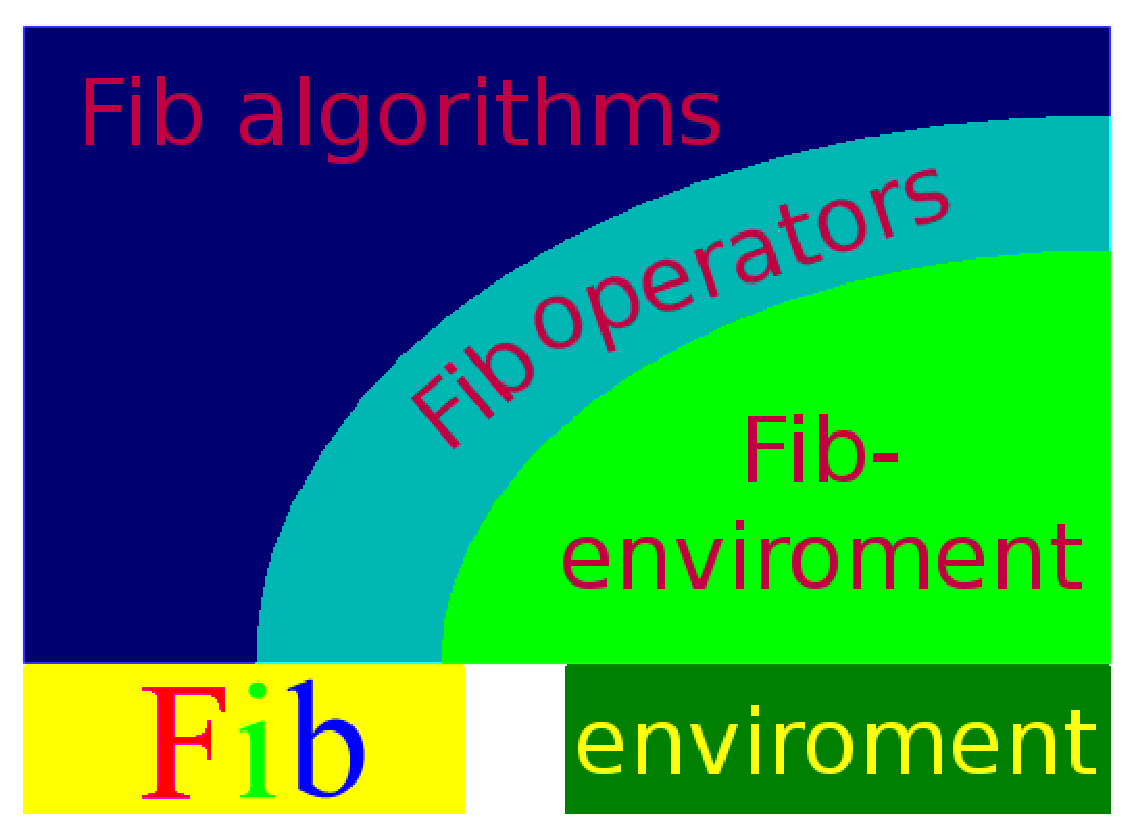
\includegraphics[scale=0.5]{project_dependencies}
\end{center}
\caption{Dependencies of the main modules}
\label{figMainModulDependencies}
\end{figure}

The ``enviroment.fib'' module requires for its individuals the Fib objects, but only as a name (for Fib objects). The ``enviroment.fib'' module thus only needs one name for Fib objects and no knowledge of the functionality (methods) of the Fib objects. Therefore the ``enviroment.fib'' module is not dependent on the ``fib'' module.

















